%% ==============================================================================
%% AASTeX v6.3.1 companion manuscript -- PRELIMINARY REDRAFT (2026-11)
%% ==============================================================================
%% Scope reduced to what the simulations in this repository deliver: the response of
%% the kilonova recovery efficiency to the selection criteria (Suite 02). All Suite 02
%% numbers are placeholders (\tbd{}) pending the ensemble re-run with the corrected
%% filter and candidate envelope. Imposter contamination is presented as planned work.
%% See docs/paper_revision_plan.md.
%% ==============================================================================

\documentclass[twocolumn]{aastex631}

\usepackage{amsmath}
\usepackage{amssymb}
\usepackage{graphicx}
\usepackage{booktabs}
\usepackage{xcolor}

\newcommand{\tbd}[1]{\textcolor{red}{[TBD: #1]}}
\newcommand{\vteff}{\langle VT\rangle}
\newcommand{\gpcyr}{\mathrm{Gpc}^{-3}\,\mathrm{yr}^{-1}}

\shorttitle{Selection Criteria for Kilonova Searches}
\shortauthors{Barna et al.}

\begin{document}

\title{How Selection Criteria Shape the Kilonova Sensitivity of Wide-Field Optical Surveys: A Systematic Study with Eight Years of ZTF}

\author[0000-0002-0000-0000]{Tyler Barna}
\affiliation{Minnesota Institute for Astrophysics, School of Physics and Astronomy, University of Minnesota, 116 Church Street SE, Minneapolis, MN 55455, USA}
\email{barna314@umn.edu}

\author{\tbd{co-authors}}

\begin{abstract}
Untargeted kilonova searches select fast transients with cuts on detection significance, the number and spacing of detections, duration, fade and rise rates, and Galactic latitude. We quantify how each cut changes the recovery efficiency, and hence the effective volume--time $\vteff$ and rate limit, of eight years of the Zwicky Transient Facility. Light curves recovered under a loose criteria envelope in $10^8$ injections per model are re-filtered on a grid of 427\,692 criteria combinations. The filter reproduces the selection of the full simulation \tbd{to X\% at the fiducial point after the re-run}. \tbd{Ranking of criteria by their effect on $\vteff$; one-at-a-time ranges; strongest pairwise interactions; recommendations.} Imposter contamination, which sets the other side of the trade-off, is outlined as the next step.
\end{abstract}

\keywords{Neutron stars (1108) --- Transient sources (1851) --- Sky surveys (1464) --- Astronomy data analysis (1858)}

%% ==============================================================================
\section{Introduction}
\label{sec:intro}

Searches for kilonovae in wide-field survey data must reject a large number of unrelated transients and artefacts \citep{Doctor2017, Andreoni2020, Andreoni2021}. The cuts used to do so also remove genuine kilonovae, so the choice of criteria sets the sensitivity of the search and the resulting rate limit. In ZTF \citep{Bellm2019, Graham2019}, the first 23 months were searched with band-dependent fade-rate cuts and without a Galactic-latitude cut \citep{Andreoni2020}. The real-time ZTFReST pipeline uses a single 0.3\,mag\,d$^{-1}$ fade threshold and $|b| > 10^\circ$ \citep{Andreoni2021}. Fast optical transients that mimic kilonovae at early times include stripped-envelope supernovae with shock-cooling peaks, which dominate a recent catalogue of ZTF kilonova imposters \citep{Barna2025}, and fast blue optical transients \citep{Ho2023}.

This paper accompanies our eight-year ZTF rate analysis \tbd{citation} and asks how strongly the recovery efficiency depends on each criterion. Section~\ref{sec:method} describes the simulate-once/filter-many method and its validation, Section~\ref{sec:results} the response of $\vteff$ to the criteria, and Section~\ref{sec:imposters} the planned contamination study.

%% ==============================================================================
\section{Method}
\label{sec:method}

\subsection{Candidate generation}
For each model (POSSIS two-component kilonovae evaluated with the \texttt{fiesta} surrogate, \citealt{Bulla2019, Bulla2023, Koehn2025}, at fixed $\iota = 25.8^\circ$ and with isotropic viewing angles; and a one-zone template), we inject $10^6$ kilonovae per realisation into the ZTF exposure history (2018--2026) with the same injection scheme as the rate paper. All recovered light curves that pass a loose envelope are stored: $\ge 1$ detection at $S/N \ge 3$, duration $\le 35$\,d, no separation or rate requirement, $|b| \ge 15^\circ$, and $z_{\max} = 0.15$. The Galactic-latitude cut is applied during simulation because positions are not stored, so the grid keeps $|b| \ge 15^\circ$ fixed. \tbd{Number of realisations per model in the ensemble re-run (target 100).}

\subsection{Criteria grid and filter}
The filter re-applies, to every stored light curve, the primary and secondary $S/N$ thresholds ($3.5$--$6.0$ and $2.0$--$4.0$), the minimum number of detections (1--5) and of primary detections (1--3), the maximum duration (2, 7, 14, 28\,d), the minimum first-to-last separation (0.5--6\,h), minimum rise and fade rates (0--1\,mag\,d$^{-1}$), and whether the rate test is required. After removing logically inconsistent combinations, 427\,692 grid points remain. Rise and fade rates are measured as in the full simulation: weighted least-squares slopes before and after the brightest point in each band, with same-band points within 2\,h averaged; a source passes if it fades or rises fast enough. $\vteff$ at each grid point is the stored efficiency times the volume--time per unit efficiency of the loose run.

\subsection{Validation}
For one realisation at the fiducial criteria ($|b| \ge 0^\circ$, rise test disabled), the full simulation recovers 2315 kilonovae and the filter 2086. With the fade requirement removed the counts agree to $\approx 2\%$. The residual difference arises because the filter measures slopes from the stored, noise-added photometry, whereas the simulation uses noiseless model magnitudes. \tbd{Validate at $\ge 5$ grid points after the re-run, and report the residual as a systematic or remove it by storing model magnitudes.}

%% ==============================================================================
\section{Response of the sensitivity to the criteria}
\label{sec:results}

\tbd{One-at-a-time response of $\vteff/\vteff^{\rm fid}$ for each criterion and model (Figure~\ref{fig:oat}); total range and local logarithmic elasticity $e = \Delta\ln\vteff/\Delta\ln x$ at the fiducial point; pairwise maps for the strongest interactions; comparison of the fiducial point with the Andreoni et al.\ (2020) and ZTFReST criteria; consequences for the rate limit.}

\begin{figure*}[t]
\centering
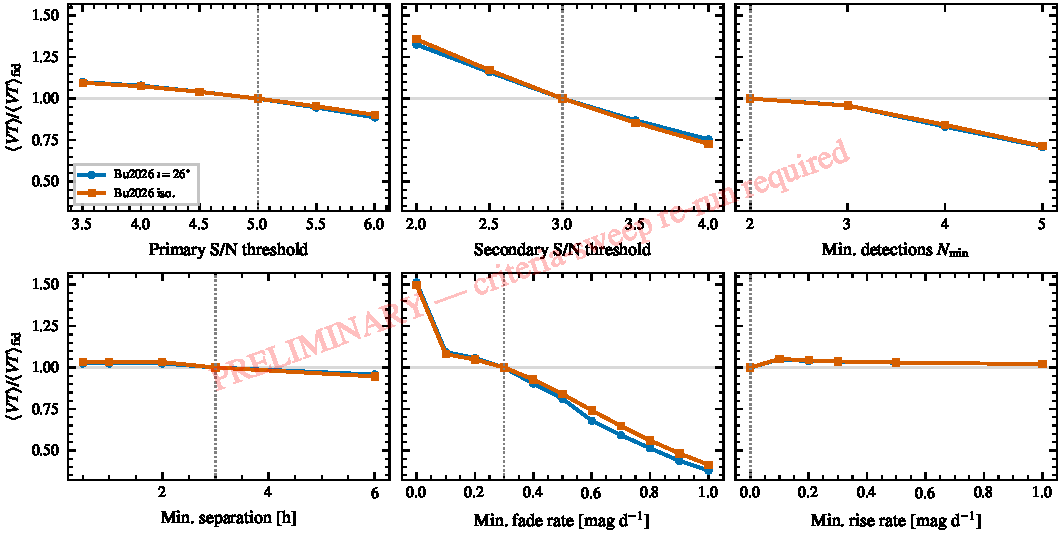
\includegraphics[width=\textwidth]{figures/fig6_criteria_sensitivity_PRELIMINARY.pdf}
\caption{\tbd{Regenerate after the re-run.} One-at-a-time response of $\vteff$, relative to the fiducial criteria (dotted lines), for each model.}
\label{fig:oat}
\end{figure*}

%% ==============================================================================
\section{Toward contamination-aware criteria}
\label{sec:imposters}

Choosing criteria requires the recovery efficiency of contaminants as well as of kilonovae. \tbd{Planned: inject shock-cooling, CSM-interaction, orphan-afterglow and cocoon light-curve models available in \texttt{survey-sim} through the same exposure history and filter; adopt volumetric rates from the literature with uncertainties; calibrate against the ZTF imposter catalogue of \citet{Barna2025}; evaluate colour-evolution discriminants on the simulated multi-band photometry; then derive completeness--purity frontiers and Rubin projections \citep[cf.][]{Andreoni2022Rubin}.} No contamination or purity numbers are given until these simulations exist.

%% ==============================================================================
\section{Summary}
\label{sec:summary}
\tbd{Summary of the criteria ranking and recommendations after the re-run.}

\begin{acknowledgments}
Based on observations obtained with the Samuel Oschin 48-inch Telescope at Palomar Observatory as part of the Zwicky Transient Facility project. Computations were performed at the Minnesota Supercomputing Institute.
\end{acknowledgments}

\software{\texttt{survey-sim}, \texttt{fiesta} \citep{Koehn2025}, \texttt{numpy}, \texttt{pandas}, \texttt{matplotlib}}

\begin{thebibliography}{}
\bibitem[Andreoni et al.(2020)]{Andreoni2020} Andreoni, I., Kool, E.~C., Sagu{\'e}s Carracedo, A., et al. 2020, ApJ, 904, 155
\bibitem[Andreoni et al.(2021)]{Andreoni2021} Andreoni, I., Coughlin, M.~W., Kool, E.~C., et al. 2021, ApJ, 918, 63
\bibitem[Andreoni et al.(2022)]{Andreoni2022Rubin} Andreoni, I., Coughlin, M.~W., Almualla, M., et al. 2022, ApJS, 258, 5
\bibitem[Barna et al.(2025)]{Barna2025} Barna, T., Fremling, C., Ahumada, T., et al. 2025, PASP, 137, 084105
\bibitem[Bellm et al.(2019)]{Bellm2019} Bellm, E.~C., Kulkarni, S.~R., Graham, M.~J., et al. 2019, PASP, 131, 018002
\bibitem[Bulla(2019)]{Bulla2019} Bulla, M. 2019, MNRAS, 489, 5037
\bibitem[Bulla(2023)]{Bulla2023} Bulla, M. 2023, MNRAS, 520, 2558
\bibitem[Doctor et al.(2017)]{Doctor2017} Doctor, Z., Kessler, R., Chen, H.~Y., et al. 2017, ApJ, 837, 57
\bibitem[Graham et al.(2019)]{Graham2019} Graham, M.~J., Kulkarni, S.~R., Bellm, E.~C., et al. 2019, PASP, 131, 078001
\bibitem[Ho et al.(2023)]{Ho2023} Ho, A.~Y.~Q., Perley, D.~A., Gal-Yam, A., et al. 2023, ApJ, 949, 120
\bibitem[Koehn et al.(2025)]{Koehn2025} Koehn, H., Wouters, T., Pang, P.~T.~H., et al. 2025, A\&A, 704, A55
\end{thebibliography}

\end{document}
